\thispagestyle{plain}
\newpage
\section{Testing}\label{sec:testing}

\normalsize

Testing for the project was a continuous process.
Given the interconnectedness of the cloud project,
components of the system needed to be deployed in a live environment so that they could be tested manually.
To enhance this process and make sure any breaking changes were captured quickly before any changes were deployed,
test automation was implemented.

\subsection{Test Automation}\label{subsec:test-automation}

Section~\ref{subsec:continuous-integration-continuous-deployment} describes how the project was set up
to automatically run tests on the system's functionality using the~\gls{playwright} framework.
Commits to the GitHub repository for the project triggered redeployment and the ability
to test changes in a cloud environment quickly in addition to running regression tests each time.
In total,
nine end-to-end tests and nine component tests were written
to ensure that the basic functionality of the software was not broken by new changes.
A screenshot of end-to-end test results can be found in~\ref{fig:playwright-results}.
Note that these tests cover the three most popular browser types: Chromium, Firefox, and Webkit.
They also incorporate visual testing through the comparison of screenshots taken of the application.
If there is any major discrepancy, the tests would fail,
helping to ensure that the deployed application remained visually consistent.
However, for the success of the project, manual testing also needed to take place.

\begin{figure}[!htb]
    \minipage{\textwidth}
    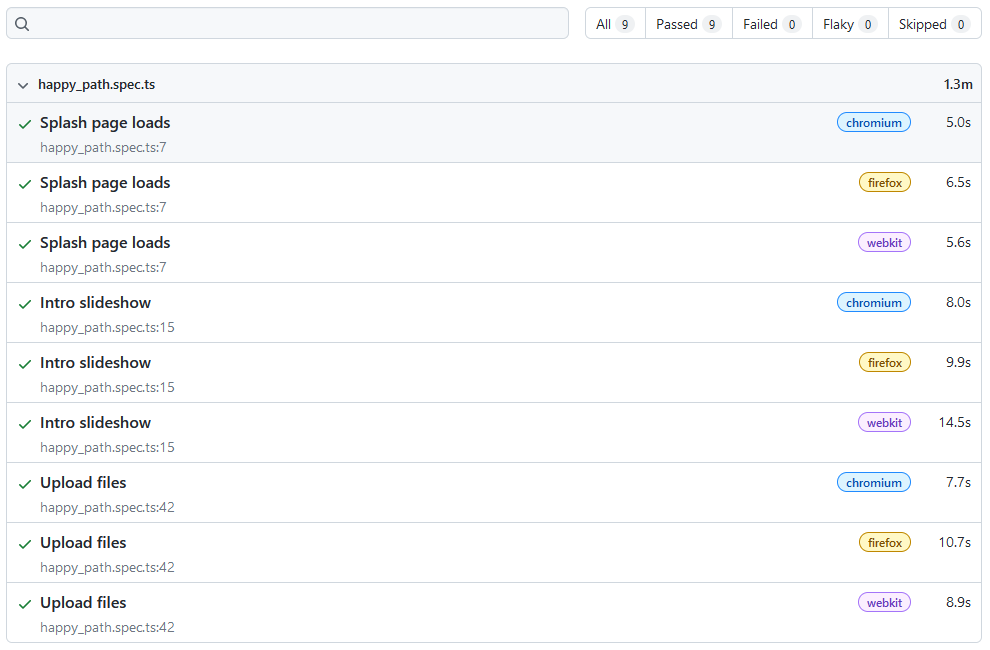
\includegraphics[width=\linewidth]{playwright-results}
    \caption{A screenshot of an HTML page produced by~\gls{playwright}. Details the passing of automated end-to-end tests}\label{fig:playwright-results}
    \endminipage
\end{figure}

\subsection{Manual Testing}\label{subsec:manual-testing}

Manual testing was required to ensure that the functionality of the service was in place.
Oftentimes, this took the form of deploying either a~\gls{docker} image
to run in~\gls{aws-lambda} or the~\gls{react} front-end to~\gls{amplify} and
then manually testing the changes that were made.
Based on the results of the manual testing, the next stage of development would be determined,
whether that be a failure in the newly deployed version, or moving onto another feature to develop.

\subsection{User Testing}\label{subsec:user-testing}

In order to identify potential issues and areas of improvement for early versions of the product,
it was important to gather feedback from users who did not have intimate knowledge of the system.

User testing was carried out
by deploying a stable early version of the system to its own~\gls{amplify} environment
and then sending out a link to that deployment along with a form that allowed testers to submit feedback.
This form was made up of questions
that solicited both qualitative and quantitative answers relating to the functionality of the system
and how easy it was to use.
Since this activity involves human participants, consideration of ethics approval was considered.
Ultimately,
this was not sought
because the nature of the research fell under one of the typical exemptions for this kind of research:

\begin{quotation}
    3.
    Service evaluation (where the following apply):
    a.
    the ‘service provider’
    or someone acting on their behalf aims primarily
    to monitor or improve a service being delivered by collecting information from a `service user'~\citep{qmul_2023};
\end{quotation}


The responses to this form can be found in Appendix~\ref{sec:appendix:-user-testing-responses}.

The response gave a gauge not only on the success of the project, but on what further revisions could be made.
All the respondents reported that the project functioned as expected with no failures reported.
Most respondents reported an increase in understanding of what spatial audio was after using the product,
however, some respondents self-reported that after having used the product,
they did not know what was meant by spatial audio, with some confusing it still with stereo audio products.

Many respondents noted
the lack of development in the~\gls{ui} and requested a better understanding
of what aspects of the program were performing which function through the use of more text or labelling.
One user reported a playback bug that was fixed in later versions,
and another requested real-time mixing of the audio signals, as in modern digital audio workstations.
Crucially,
all respondents stated
that they did not have access to the same kind of spatial audio technology that was offered by the product.
This meant that the project was successful in increasing access to customisable spatial audio.

Requested features from testing:

\begin{itemize}
    \item A graphical user interface (Implemented).
    \item Loading bar for separation progress.
    \item Loading bar for~\gls{stem} playback (Implemented).
    \item Guidance for playing around with the product's sliders.
    \item Live feedback on spatial positions (Implemented).
    \item Synchronised playback of~\glspl{stem} (Implemented).
    \item Mute and solo buttons for each~\gls{stem} during playback (Implemented).
    \item Tidying of layout and formatting (Implemented).
    \item Loading screen when uploading files (Implemented).
\end{itemize}

Having these requests made it easy to make improvements to the product that would improve the~\gls{ux}.
It also resulted in a greatly improved final product.

\subsection{Lines of Code}\label{subsec:lines-of-code}

While the total lines of code in a project are not evidence of its complexity or completeness,
a report was run on the files in the repository for the sake of completeness.

The output of the code report can be found in Listing~\ref{lst:loc-output}.

\begin{longlisting}
    \inputminted[
        breaklines,
        frame=lines,
        framesep=2mm,
        baselinestretch=1.2,
        fontsize=\footnotesize,
        linenos,
    ]{output}{../../cloc_output.txt}
    \caption{Lines of code per file type in the project repository}\label{lst:loc-output}
\end{longlisting}
